\documentclass[sigconf]{acmart}
\usepackage{booktabs}
\usepackage{xcolor}
\usepackage{graphicx}


%% \BibTeX command to typeset BibTeX logo in the docs
\AtBeginDocument{%
  \providecommand\BibTeX{{%
    \normalfont B\kern-0.5em{\scshape i\kern-0.25em b}\kern-0.8em\TeX}}}

%% These commands are for a PROCEEDINGS abstract or paper.
\settopmatter{printacmref=false} % Removes citation information below abstract
\renewcommand\footnotetextcopyrightpermission[1]{} % removes footnote with conference information in 

\acmConference[AEPRO 2024]{AEPRO 2024: Algorithm Engineering Projects}{March 1}{Jena, Germany}

% convert text to title case
% http://individed.com/code/to-title-case/

% that helps you to formulate your sentences
% https://www.deepl.com/translator

\begin{document}

%%
%% The "title" command has an optional parameter,
%% allowing the author to define a "short title" to be used in page headers.
\title[Project 1: Enhancer for Scanned Images]{Project 1: Enhancer for Scanned Images\\\large Algorithm Engineering 2024 Project Paper}

%%
%% The "author" command and its associated commands are used to define
%% the authors and their affiliations.

\author{Onur Yilmazer}
\affiliation{%
  \institution{Friedrich Schiller University Jena}
  \country{Germany}}
\email{onur.yilmazer@uni-jena.de}

\author{Lisa Kim Will}
\affiliation{%
  \institution{Friedrich Schiller University Jena}
  \country{Germany}}
\email{lisa.will@uni-jena.de}

%% The abstract is a short summary of the work to be presented in the article.

\begin{abstract}

In our pursuit of improving document quality and readability, we were motivated to develop an efficient program, which focuses on enhancing scanned documents. Drawing inspiration from the three given key papers on 'adaptive thresholding', namely 'Adaptive Thresholding Using the Integral Image', 'Binarization of historical document images using the local maximum and minimum', and 'Adaptive Thresholding Methods for Documents Image Binarization', our implemented techniques address image editing needs like noise reduction, background removal, and contrast enhancement. Our program prioritizes efficiency in both time and storage usage, as well as portability and a user-friendly interface. This paper details how the input color image(s) in JPG, PNG and BMP formats are being processed into the cleaned image(s) in JPG format, our chosen method for adaptive thresholding, specifically utilizing the integral image technique and our thoughts behind optimizations.

\end{abstract}

%%
%% Keywords. The author(s) should pick words that accurately describe
%% the work being presented. Separate the keywords with commas.
\keywords{noise reduction, background removal, image filter, adaptive thresholding}


%%
%% This command processes the author and affiliation and title
%% information and builds the first part of the formatted document.
\maketitle

\let\thefootnote\relax\footnotetext{AEPRO\textcolor{red}{?} 2024, March 1, Jena, Germany. Copyright \copyright 2024 for this paper by its authors. Use permitted under Creative Commons License Attribution 4.0 International (CC BY 4.0).}



\section{Introduction}

\subsection{Background}

 Enhancing the quality of scanned documents is a direct application of the field computer vision and graphics. Depending on the chosen methods, it may involve steps such as converting the input image into grayscale and applying various algorithms to improve readability. Techniques such as image denoising, contrast enhancement, and edge detection are being applied with the goal to reach a high contrast image in which the text is well readable in deep black in front of a white clean background with as little as possible disturbances. Our project focuses on thresholding to achieve this, which means that we try to classify pixels as either “dark” or “light”, of course with the goal that text pixels are classified as dark, while the background pixels get classified as light. Now there are different ways to apply thresholding. The most simple and straight forward technique is to choose a fixed threshold value and compare each pixel to it. However, when the illumination differs locally throughout the image it often fails \cite{LecSource2}. An intuitive measurement to overcome this issue is to find a way to compute the threshold value locally. This approach is called "Adaptive Thresholding", since we adapt the value to the varying illumination throughout the image.

\subsection{Related Work}

In the paper "Adaptive Thresholding Using the Integral Image", Derek Bradley and Gerhard Roth present a technique to calculate the sum of the locally surrounding pixels of the one we are looking at, the so called "Integral Image" and then weigh the given threshold with it. That means that the threshold value is calculated for each pixel individually, which is the special thing about their presented method, that piqued our interest most. Their paper focuses mainly on the theoretical details of the method and not the practical application.

\subsection{Our Contributions}

Our work focuses on adapting Derek Bradley and Gerhard Roth's technique for practical usage and integrating it in a project with an intuitive interface for end-users. Their particular technique is the fundamental algorithm of our project, which involves creating an executable with the purpose of enhancing the quality of text documents. On the occasion of the topics of our course, which evolve around efficiency and portability of code, we did lay focus on implementing the task in a way that allows a fast and reliable conversion of the input images to well readable output images. We placed emphasis on parallelizing our main algorithms for faster execution times. During our testing phase, we created multiple benchmarks to see which parallelization techniques resulted in the biggest performance gains and set the default parameters of our executable accordingly.

\subsection{Outline}

The paper will be structured as follows. The reader will first be introduced to the algorithms that our program is based upon, namely grayscale conversion and adaptive thresholding with the Integral Image. We will explain how exactly they work, how we implemented them and if applicable how we tried making them more efficient. After that we will present the benchmark experiments that we implemented and discuss their results. Last but not least we will finish our work with a conclusion.

\section{The Algorithms}

As mentioned, the processing of the given images consist of two algorithms. First we convert the input data into grayscale data, if they are not already in that format. After that we apply adaptive thresholding on the data, which is the important part and focus of our work. 

\subsection{Converting into Grayscale/ Preprocessing}

At this point I want to mention, that since we are using the stb library, our conversion doesn't take place manually on the raw image data. Instead we use $stbi\_load()$ on each file and apply all algorithms on the contained data. However the image data remains still in the familiar order. The color component values per pixel, which will be of interest, are stored in the order red, green, blue. With convertToGrayscale() we will forge the three color values into one which is for our eye something between or black and white. To do that, we add the red, blue and green values and divide by 3. \\

Let us now take a closer look at the implementation of this algorithm. First of all, it is to be mentioned, that we took into consideration, that one pixel can contain of more than the red, green and blue values, e.g. brightness, therefore we do not increment by three but by the nrOfChannels. Next I want to point out, that our convertToGrayscale()-function is being called within the function that handles the adaptive thresholding, namely applyAdaptiveThresholding(). We only call the convertToGrayscale()-function, if the image is not already in grayscale. applyAdaptiveThresholding() on the other hand is being called in processFolder() within a parallel region, which is to be considered when trying to parallelize the convertToGrayscale()-function. In order to enable another parallel region, we call "$omp\_set\_nested(1)$". We assign each thread the same amount of pixels to work on, namely $\frac{\#PixelsInTotal}{\#Threads}$. The master thread takes care of the leftover pixels that represent the rest of the division. Now within the parallel region, each thread takes care of its assigned work. 

\subsection{Applying Adaptive Thresholding}

The first part of this function evolves around creating the integral image, which is in general also called "Summed-area table". For each pixel, the integral image entry is calculated as follows:\cite{LecSource2}

\begin{equation}
{\displaystyle I(x,y)=i(x,y)+I(x,y-1)+I(x-1,y)-I(x-1,y-1)}
\end{equation}

where $i(x,y)$ is the original pixel value in the spot we look at. We add to it the integral image entry of the position one above and one to the left and subtract the one from diagonally to the top left. As a result we get an array with the same amount of entries as pixels in our grayscale image. This look-up-table will come in handy later, when we need to calculate the sum of values within smaller windows of our image. Consider we want to calculate the sum of all pixels within a rectangle D as visualized in Figure 1, which is surrounded by the rectangles A, B and C, which are sandwiched between D and the image boarders.
Now one can quickly calculate the desired sum as follows:

\begin{equation}
{\sum _{\substack{x_{1}<x\leq x_{2}\\y_{1}<y\leq 
y_{2}}}i(x,y)} = I(D)+I(A)-I(B)-I(C) 
\end{equation}

where $A = (x1, y1), B = (x2, y1), C = (x1, y2) \text{ and } D = (x2, y2)$.\cite{IntImg}

\begin{figure}[htbp]
  \centering
  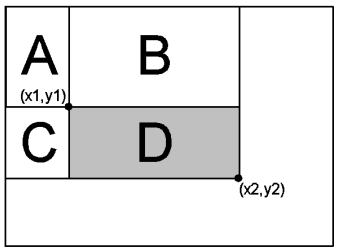
\includegraphics[width=0.7\linewidth]{./graphics/rectangle.png}
  \caption{Visualization of how integral image is used to calculate the sum over rectangle D} 
\end{figure}


We implement the integral sum a bit more efficiently than if one would implement equation (1) naively. We iterate over the columns, and within a column row-wise within the inner loop. The variable "index" describes the current position in the 1-dimensional IntegralImage-Array in regard to the position in the image matrix. The current IntegralImage-value gets calculated by adding the IntegralImage-value to its left and the sum of all column elements above including itself. The reason for not having to subtract the diagonal IntegralImage-value $I(x-1,y-1)$ is that we do not add the above IntegralImage-value, which would include that exact value, but instead the columnSum. So we do reach the same values but with a slightly changed path.\\
At this point we want to say some words about our access-pattern. Matrices are stored in row-major order by default in our language of implementation, which is C++, and this means that each time we access a matrix entry below the current one, we jump ahead N elements in the memory, with N being the width of our image. This creates an N-Stride pattern and that is highly inefficient compared to a 1-Stride pattern where contents of the memory are read consecutively. Technically, this problem could easily be solved by saving the image data in column-major format, but we use a library called "STB"\cite{std} to load image data into matrices in our program, and this library currently doesn't provide an option to do that. To keep the scope of our research limited to a reasonable size, we opted not to delve further into this optimization, but this can be a topic for further research in this area. \\

After having this useful feature implemented, we reach the heart of our program, the binarization of the pixels. With binarization we mean that we will set the current pixel value, that lies between 0 and the 255, to either 0 or the 255 based on its personal threshold value. Once again we iterate over all columns and in the inner loop through all rows and set the index to the according element in the array in which we will save the new pixel value, namely "binarized".  The size of the window we will lay around our current pixel is called $windowSize\_pixels$. We can visualize the current situation as in Figure D. In the middle of D lays our pixel of interest. Now with the already calculated Integral Images we can easily apply equation (2) in order to get the sum of all pixels in D. The same way we access the right index for binarized, we also access the right position of the integralImage-Array and save the result of the solved equation as intensitySum.\\
We now have everything prepared for the crucial decision whether our current pixel will turn black or white. \\

The pixel will be black, meaning set to 255, if its current pixel value multiplied by nrOfPixelsInWindow is bigger than intensitySum times 1 minus the given threshold-percentage. If that inequation does not hold, it will be white, meaning set to 0.\\

As one can see, we did not parallelize the applyAdaptiveThresholding()-function. But as previously mentioned, the function gets called within the already parallel processFolder()-function in "BatchProcessor.cpp". In that region we deal with images out of the directory in parallel, which means, that a thread that is available takes an image from the array we created and applies all processing on it, while other threads execute the same job on different files. Our reasoning for not implementing more parallelism within the function are as follows. The calculation of the Integral Image is hard to parallelize and not worth the effort, because each iteration is dependent of the results of previous ones. One would probably have to apply some wave-front approach with several locks, which would definitely create a too big overhead. Moving on to the next nested for-loop, which is responsible for binarization, we notice that we do not have that issue anymore and it could therefore be parallelized. However as previously mentioned, the applyAdaptiveThresholding()-function gets called within the already parallel processFolder()-function in "BatchProcessor.cpp". In that region we deal with images out of the directory in parallel, which means, that a thread that is available takes an image from the array we created and applies all processing on it, while other threads execute the same job on different files. 




\section{Experiments}

\subsection{Benchmark Environment}

All following results have been accomplished under this benchmark environment:

\begin{itemize}
    \item OS: Windows 11 version 23H2
    \item CPU: Intel® Core™ i5-11300H Processor 3.1 GHz, 4 cores (8 logical processors)
    \item RAM: 2x8 GB DDR4 SODIMM @3200MHz
    \item Compiler: g++.exe (Rev10, Built by MSYS2 project) 11.2.0
\end{itemize}



\subsection{Benchmarking applyAdaptiveThresholding()}

Our first experiment involves the question of how the runtime of the applyAdaptiveThresholding()-function on an input folder of images is dependent on the amount of threads we use. On top of that we were interested in whether parallelizing the convertToGrayscale()-function is actually worth it in the bigger picture. On that occasion we benchmarked applyAdaptiveThresholding() twice. Once with our initial sequential version of convertToGrayscale() and once with the current "optimized" parallel version. The results of all experiments can be viewed in the Appendix. The loops in our benchmark$\_$nrOfThreads()-function generally iterate over the amount of threads. We start with 1 thread and increase the number of threads up to two times the amount of logical cores, which is in our case eight, so from 1 to 16, which is reflected on the x-axis of the graphs. On the y-axis we can see the runtime. We always display two curves within the graphs: an orange one for the debug version and a turquoise one for the release version.

\subsubsection{With sequential convertToGrayscale()} 

\text{   }\\
Let us first look at the release version, which means that the code has been optimized by the compiler and all debug information gathering is disabled. So we do expect it to be much faster than the debug version, which is visibly the case in all three experiments. When running applyAdaptiveThresholding() with one thread, we have a runtime of 1.658 seconds (The concrete values are all stored within the csv-files under "benchmarks"). The runtime then steadily decreases until it settles quite fast at 4 and more threads at around 0.55 seconds. \\
Considering the debug version, meaning the version that contains all the symbolic information which is used for debugging and has code optimization disabled, the curve starts up very high at a runtime of 4.988 seconds with one thread. After that it falls faster than the the release curve until it reaches an almost constant state at an approximate runtime of 1.35 seconds starting at 6 threads. 

\subsubsection{With parallel convertToGrayscale()}

\text{   }\\
Lets us now observe the results of the applyAdaptiveThresholding()-function with the parallel sub function convertToGrayscale(), which can be viewed in Figure 3. When merely looking at the graphs, they do look surprisingly similar. The line of the release version behaves pretty much the same as the previous one. It starts off almost the same at settles after 4 threads at a runtime of 0.598 seconds. 
In the debug version the runtime also starts quite high with 5.207 seconds on one thread and also settles as well at around 6 threads and stays approximately at a runtime of 1.32 seconds.

\subsection{Benchmarking parallel convertToGrayscale()}

Considering the fact, that the parallelity didn't seem to have much of an impact on the performance, we decided to benchmark the parallel convertToGrayscale()-function separately. The resulting graph can be viewed in Figure 4. When looking at it, we do get the feedback we expected. Apparently the implementation of parallelity has almost no effect on the runtime at all. The line that displays the release version, which is more of interest and should show a more reliable pattern, if one exists, is steadily around 1 second with a very small variance. The line of the debug version does vary more, but we would not say that a pattern exists. Of course once again the mean runtime is approximately 4.4 seconds, so the debug version is 4 times slower. 

\subsection{Discussion}

The results of our experiments did not display the speed-up of parallelization we were hoping to see, however it also didn't make us slower neither, which is why we decided to keep the parallelized version in our program. It is worth pointing out, that in the benchmark results of the applyAdaptiveThresholding()-function we can see that typical behavior one would expect in a runtime $\sim\#$threads graph. With the amount of threads growing, the runtime gets shorter until it reaches a point where the limits of parallelity are reached. In our case that limit is between 4 and 6 threads, depending on the version. We strongly suggest, that this is because our environment has 4 physical cores. After 8 threads, which is the amount of logical cores, the runtime once and for all reached its limit and shouldn't go significantly lower anymore.\\
Considering the unusual behavior of the convertToGrayscale()-function, we assume that this is due to the small filesize of the images and the fact that dividing such small files among different CPU cores creates cache-related problems. 


\section{Conclusions}

Looking back at our work, we believe that we were able to accomplish our goal of developing an efficient and reliable program to improve quality and readability of scanned documents, and we are satisfied with our results. An example follows:\\

\begin{figure}[htbp]
  \centering
    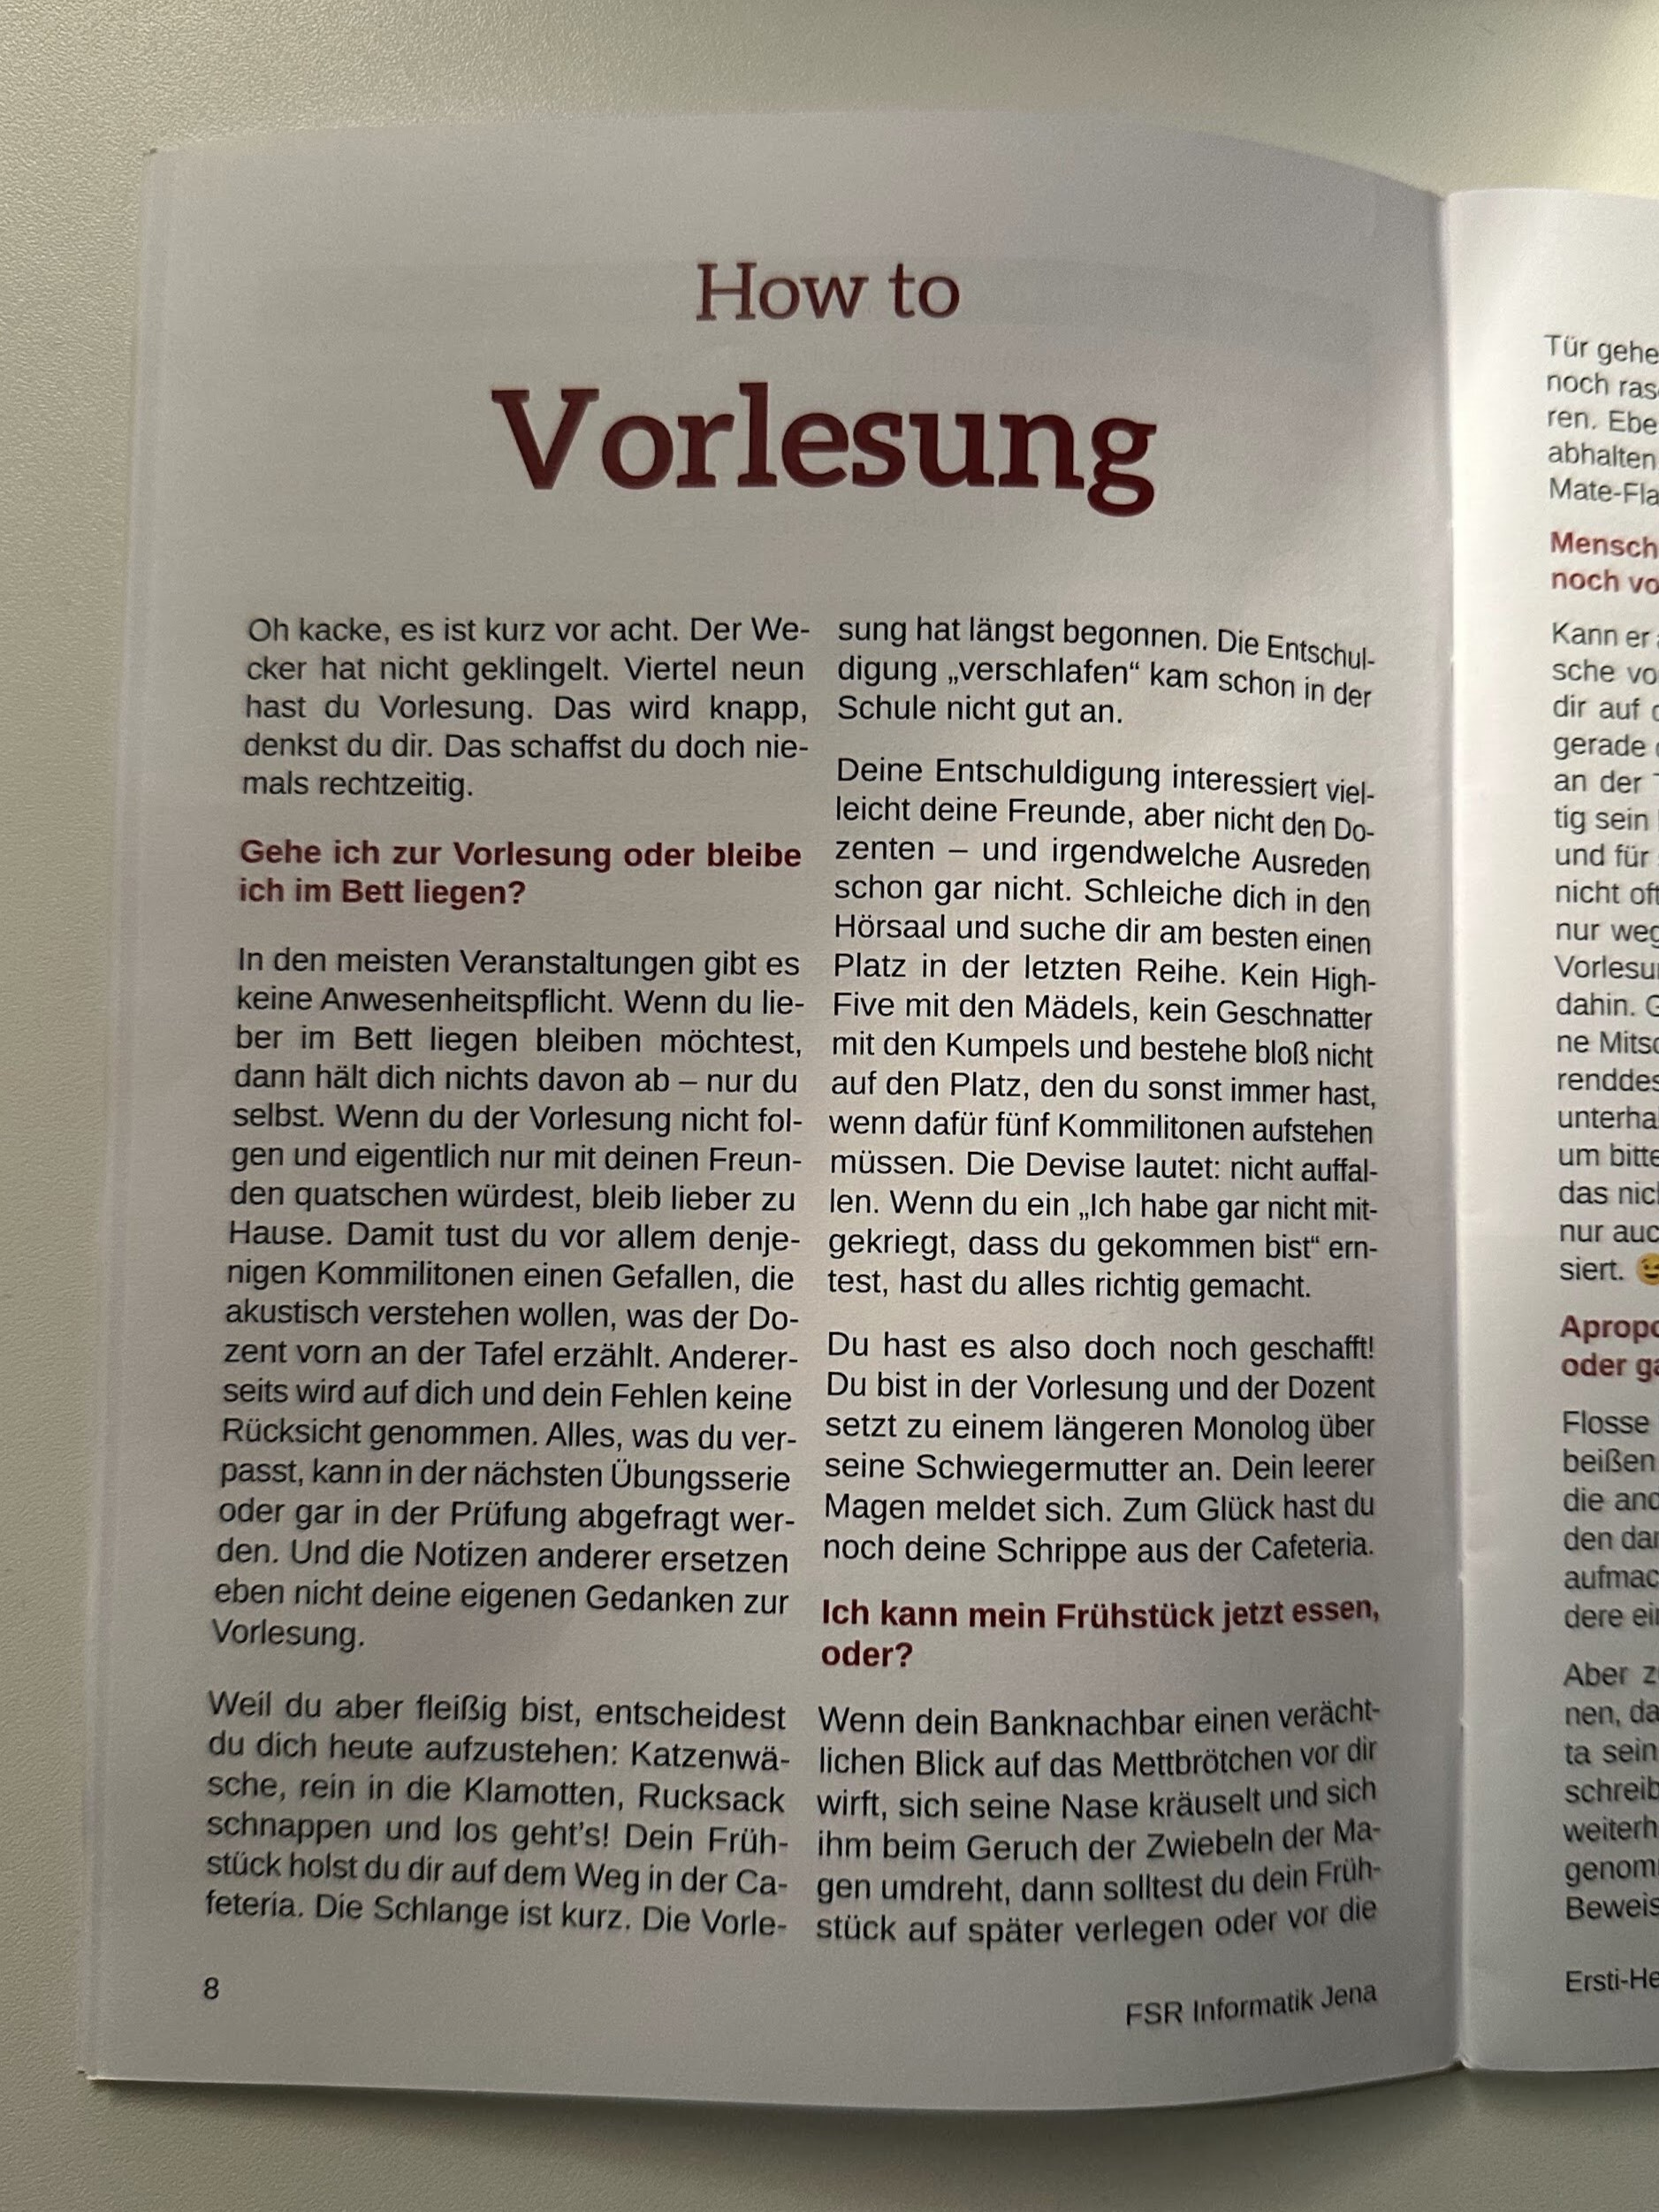
\includegraphics[width=0.45\linewidth]{./graphics/heft_4.jpg} 
    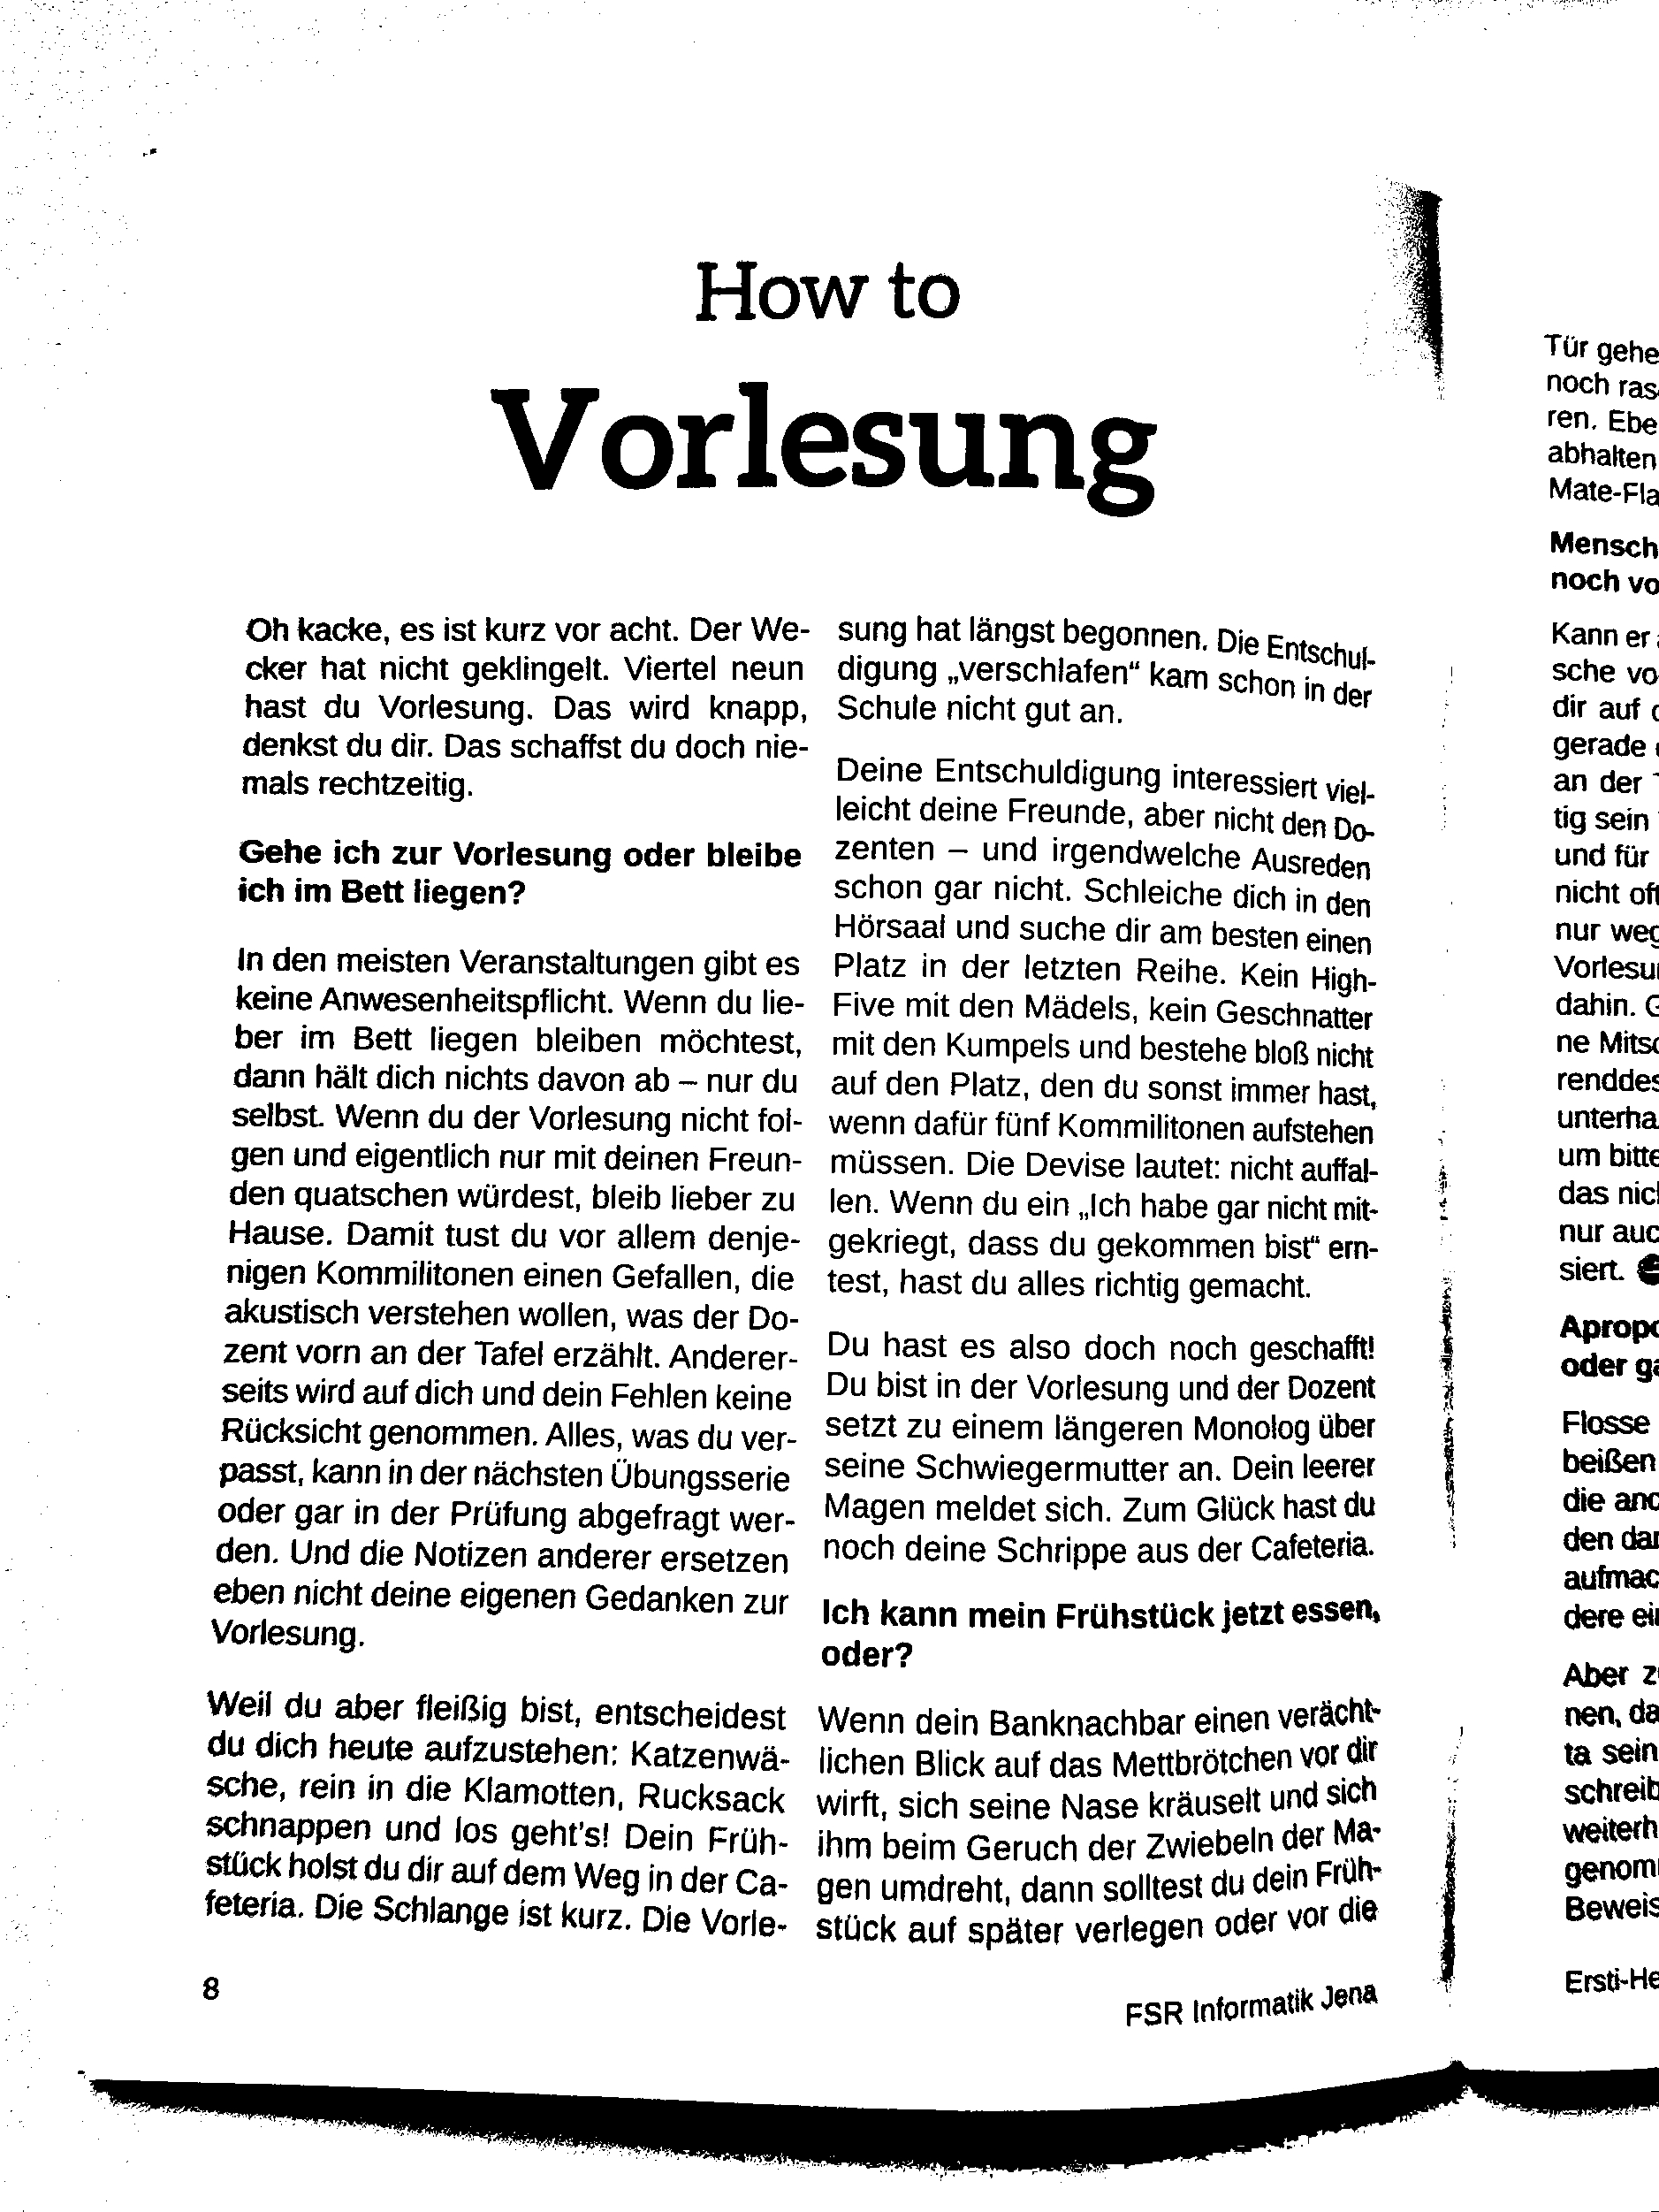
\includegraphics[width=0.45\linewidth]{./graphics/heft_4_binarized.jpg} 
    \caption{Image before and after processing}
\end{figure}

The global parallelity enables a fast execution. Of course we are a bit disappointed that we couldn't apply more parallelity on a more local level, but since we did try and benchmarked it, we assume that we are not missing out too much.\\
The integral image proved itself to be a useful technique for image processing. We believe it might come in handy in other projects in the future since its application is a recurring task in many problem statements. Based on our resulting images we would say, that we empowered the reputation of the presented algorithm that was discussed in the paper "Adaptive Thresholding Using the Integral Image". 


%%
%% The next two lines define the bibliography style to be used, and
%% the bibliography file.
\begin{thebibliography}{h}
\bibitem{LecSource2}Derek Bradley, Gerhard Roth. Adaptive Thresholding Using the Integral Image, Journal of Graphics GPU and Game Tool, 2007
\bibitem{IntImg}Username: BADGERATI, Computer Vision – The Integral Image, https://computersciencesource.wordpress.com/2010/09/03/computer-vision-the-integral-image/, 2010, (Last access date: 12.03.2024)
\bibitem{stb}Sean Barrett, "stb single-file public domain libraries for C/C++", https://github.com/nothings/stb, (Last access date: 14.03.2024)

\end{thebibliography}

\newpage

\onecolumn
\section{Appendix}

\begin{figure}[h]
  \centering
  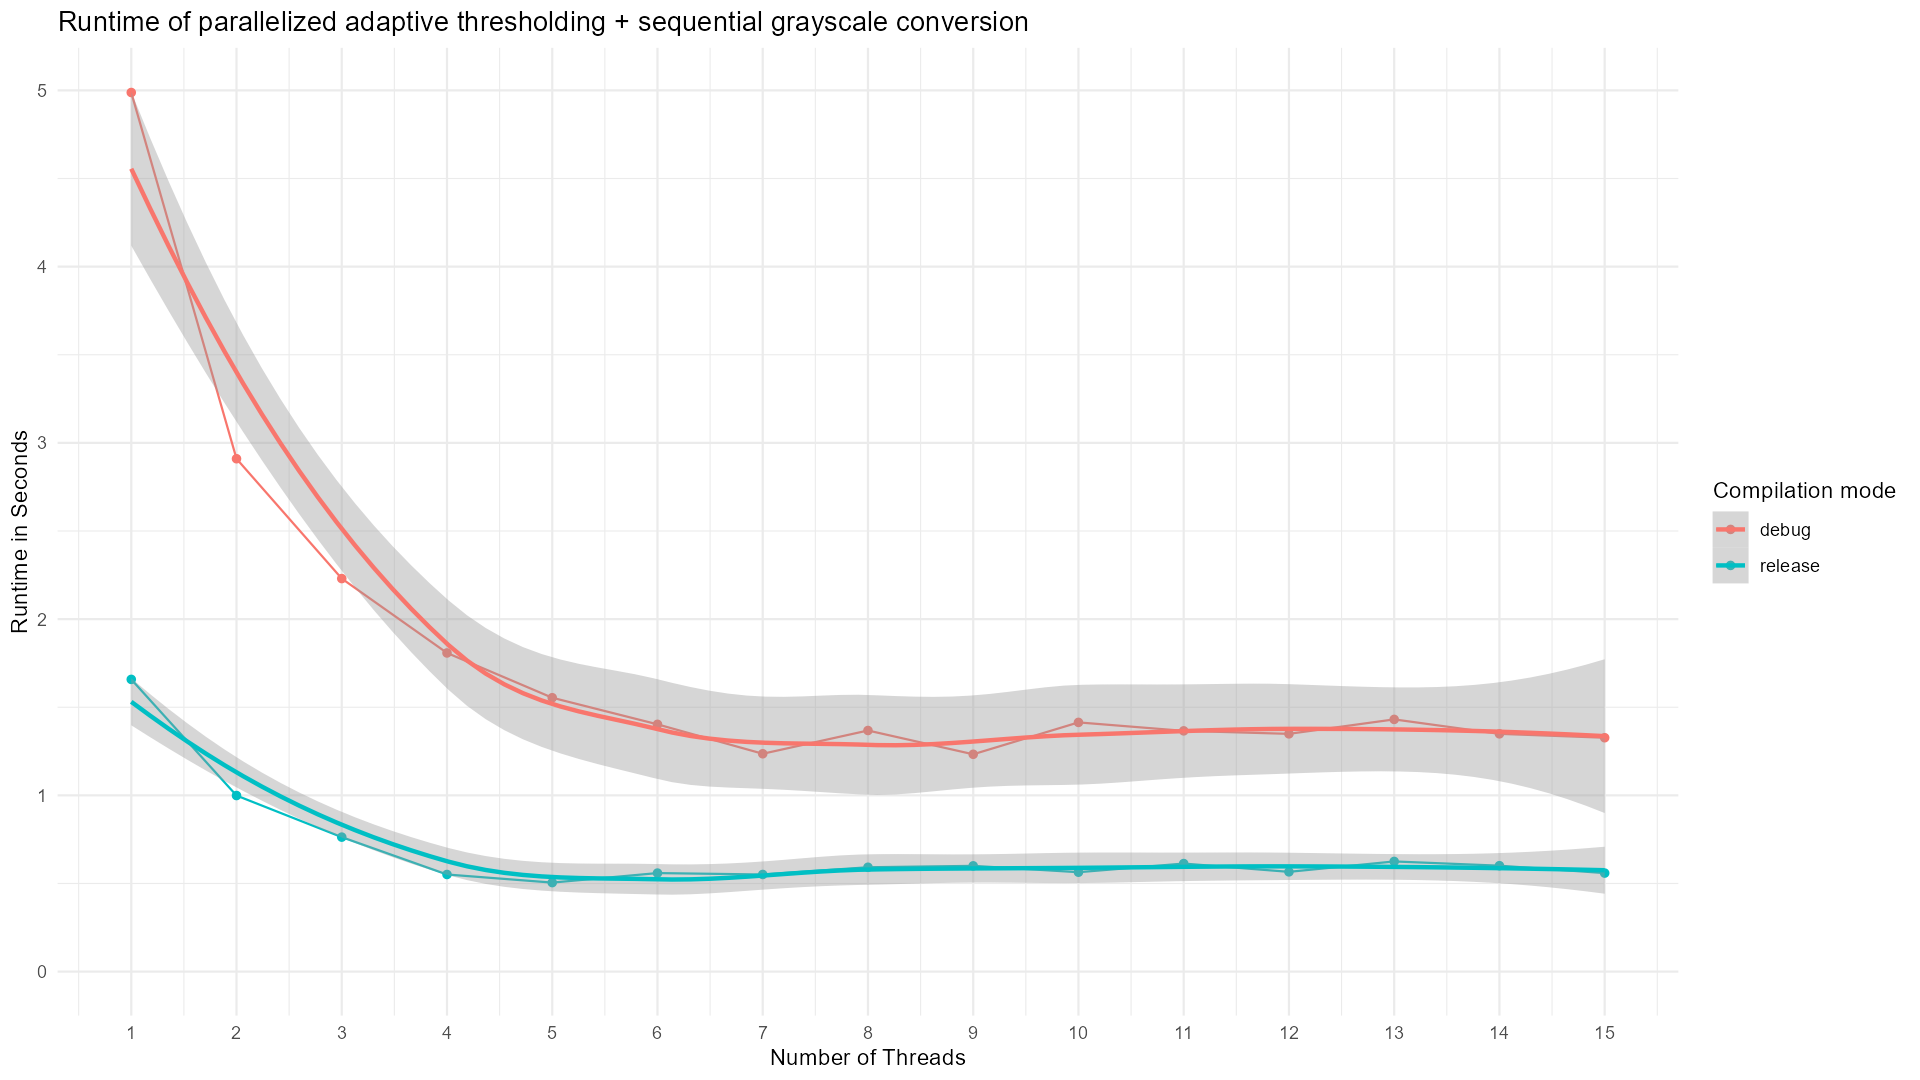
\includegraphics[width=0.9\textwidth]{./graphics/paralleladaptive_sequentialgrayscale_benchmark.png}
  \caption{Benchmarking AdaptiveThresholding with sequential GrayscaleConversion} 
\end{figure}

\begin{figure}[h]
  \centering
  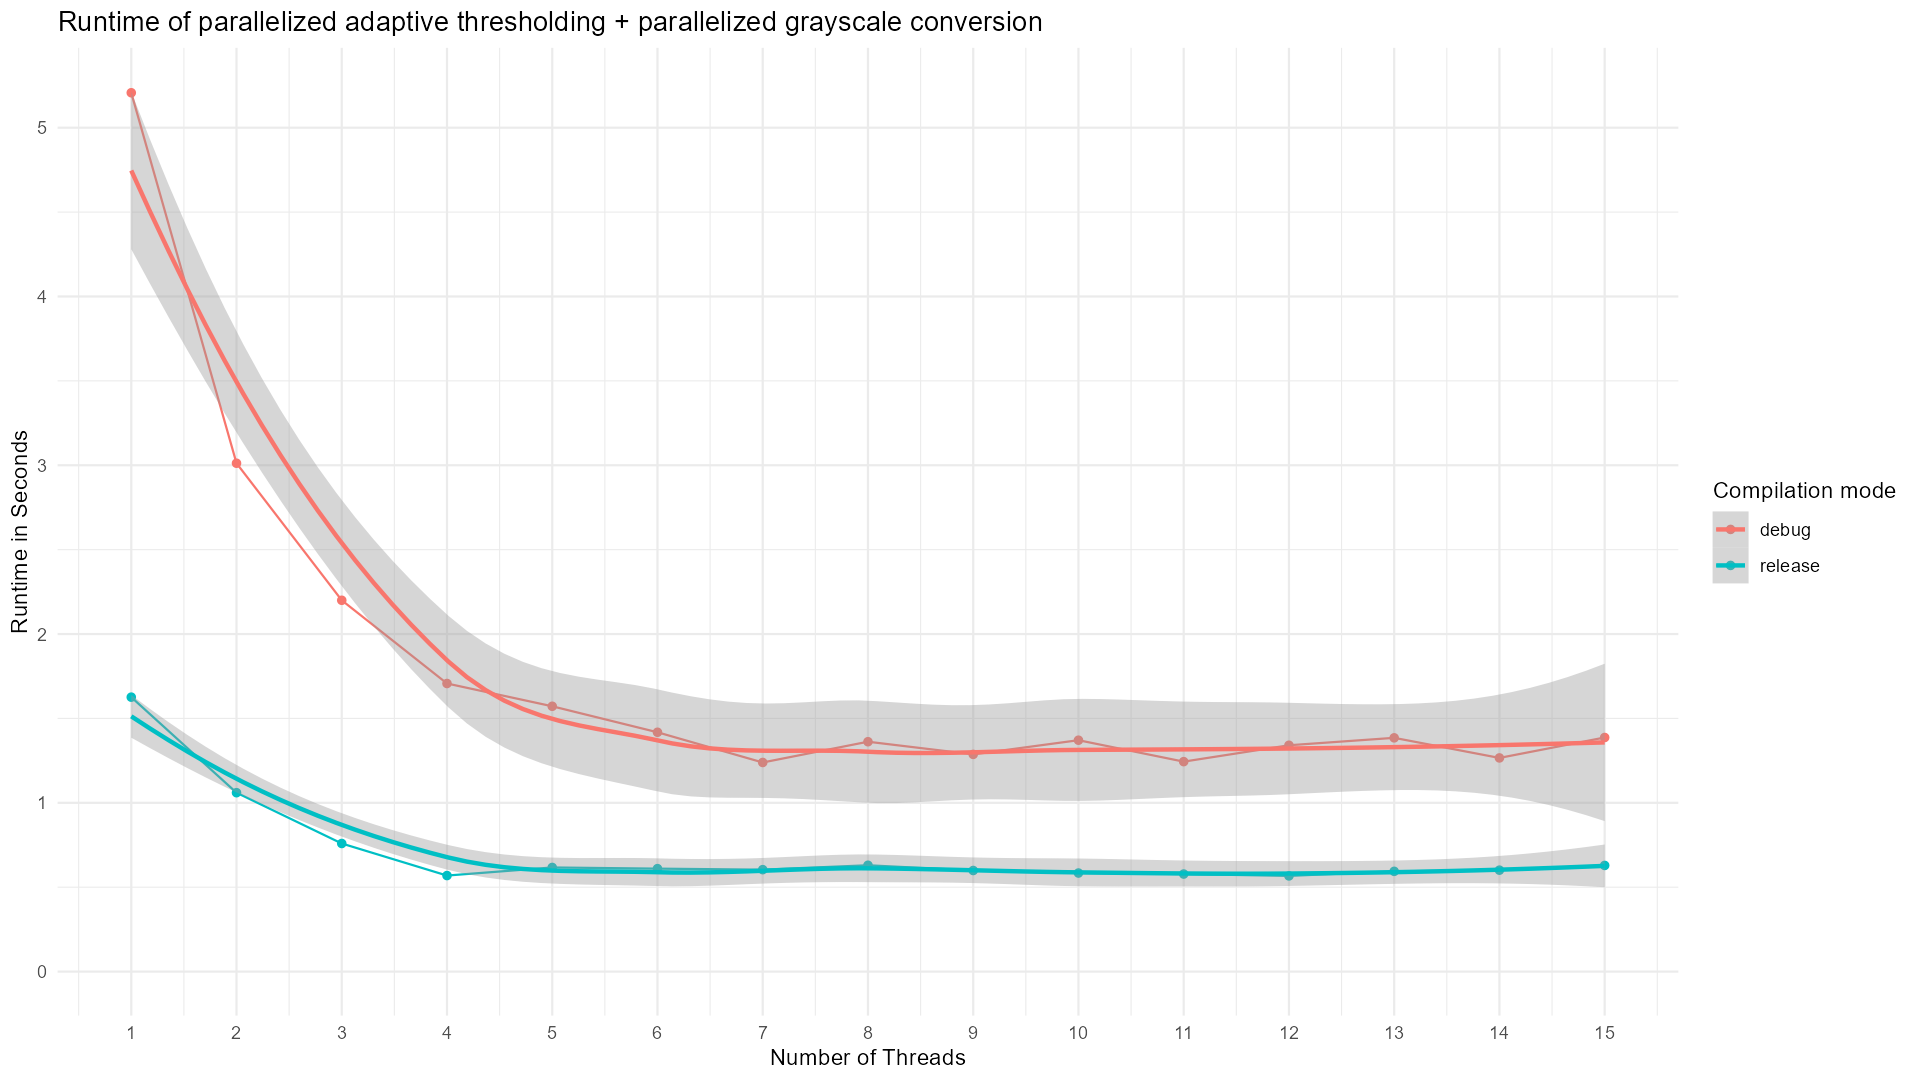
\includegraphics[width=0.9\textwidth]{./graphics/paralleladaptive_parallelgrayscale_benchmark.png}
  \caption{Benchmarking AdaptiveThresholding with parallel GrayscaleConversion} 
\end{figure}

\begin{figure}[h]
  \centering
  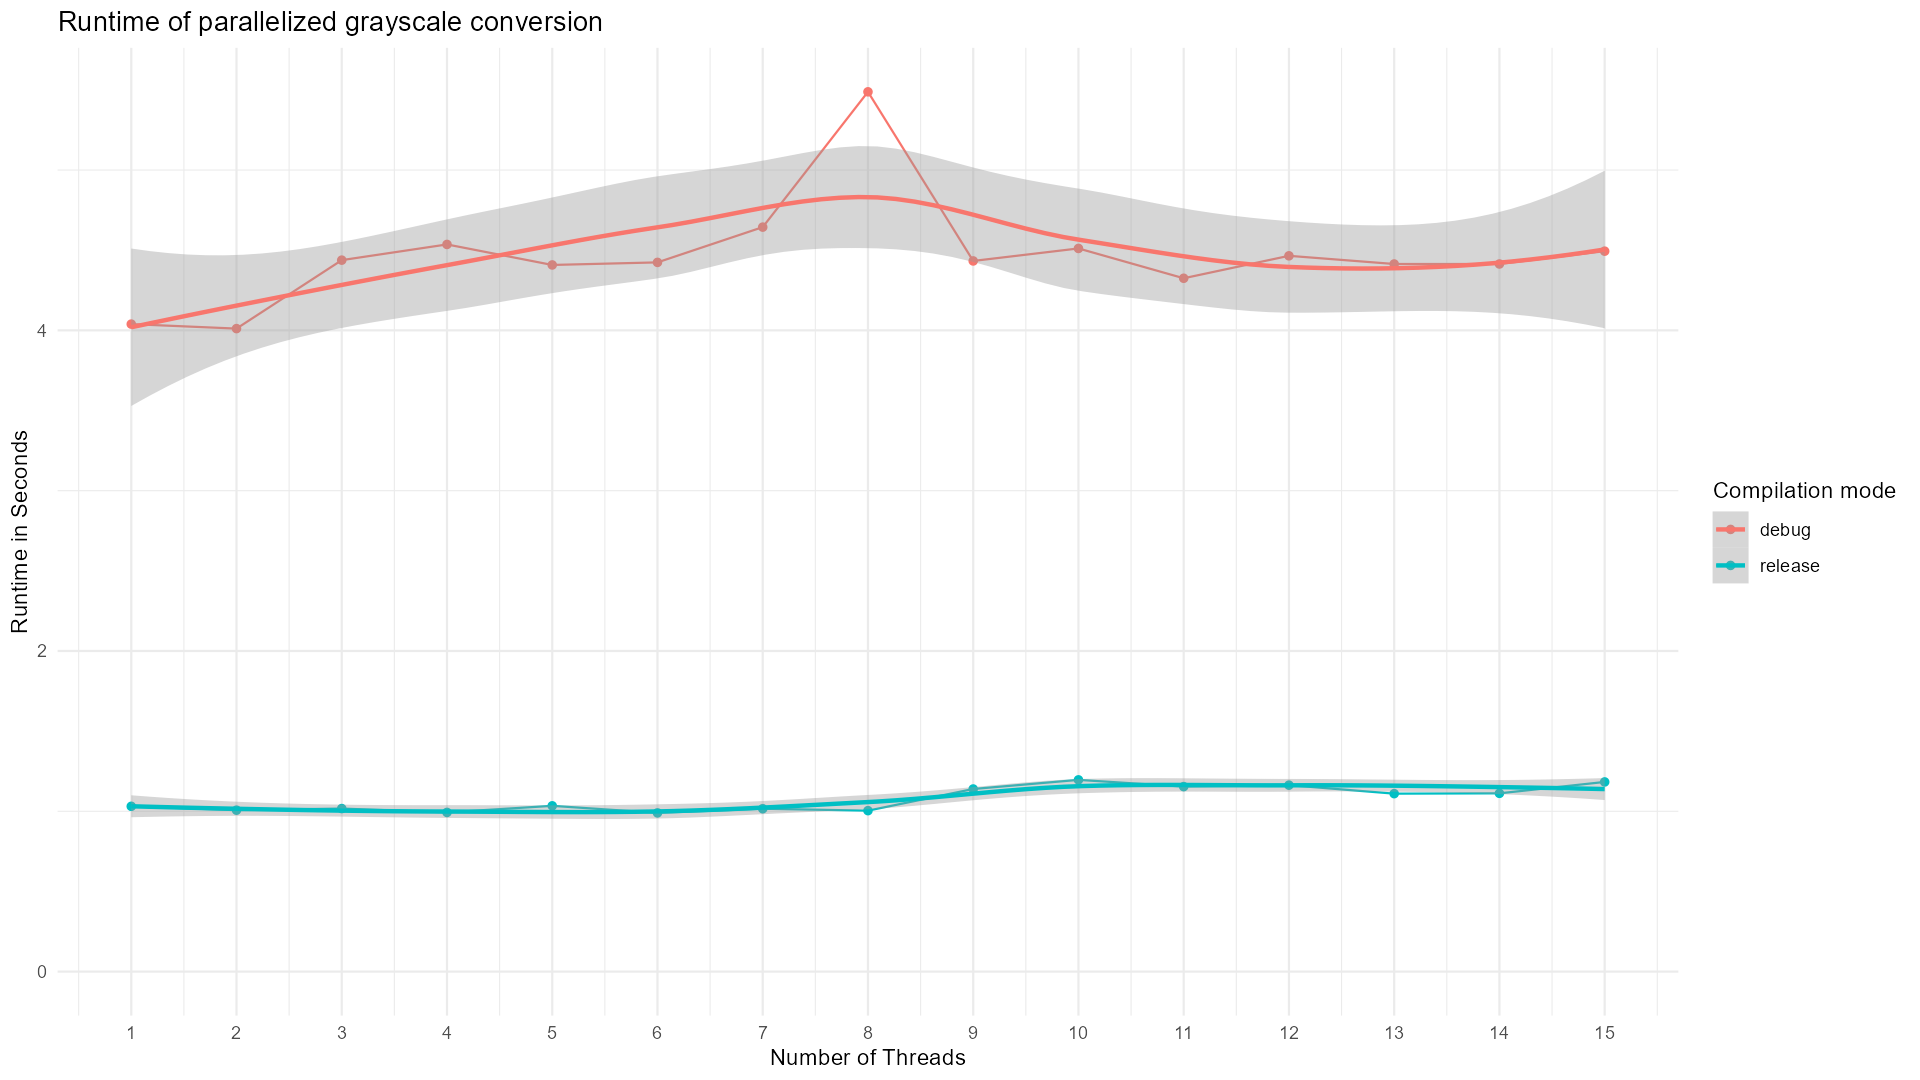
\includegraphics[width=0.9\textwidth]{./graphics/parallelgrayscale_benchmark.png}
  \caption{Benchmarking parallel GrayscaleConversion separately} 
\end{figure}



\end{document}
\endinput
%%
%% End of file `sample-sigconf.tex'.
